\documentclass[a4paper,12pt]{article}

\usepackage{amssymb,amsmath} %math symbols

\usepackage[margin=2cm]{geometry} %paper geometry

\usepackage[T1, T2A]{fontenc} % T2A for Cyrillic font encoding
\usepackage[english, russian]{babel}
\usepackage[russian]{babel} %docment in russian-style
\usepackage[utf8]{inputenc}
\usepackage[unicode]{hyperref} %links inside of the text
\usepackage[pdftex]{graphicx} %includegraphics pictures
\usepackage{cmlgc} %bold text

\usepackage{array} %arrays

\usepackage{wrapfig}
\usepackage{array}
\usepackage{lipsum}
\usepackage{esvect}
\usepackage{hyperref}
\usepackage{xcolor}
\definecolor{linkcolor}{HTML}{799B03} % цвет ссылок
\definecolor{urlcolor}{HTML}{799B03} % цвет гиперссылок
 
\hypersetup{pdfstartview=FitH,  linkcolor=linkcolor,urlcolor=urlcolor, colorlinks=true}
 
\usepackage{subfig}
\usepackage{calc}
\usepackage{pgfplots,tikz,circuitikz}
\usepackage{pgfplotstable}
\usepackage{tkz-euclide}

\usepackage{centernot}
\usepackage{cancel}

\documentclass{article}
\usepackage{amsmath}
\usepackage{mathtext}
\usepackage[T1,T2a]{fontenc}
\usepackage[utf8]{inputenc}
\usepackage[english, bulgarian, russian]{babel}
\usepackage{tikz}
\usepackage{pgfplots}
\usepackage[export]{adjustbox}
\usepackage[left=2cm,right=2cm,
    top=2cm,bottom=2cm,bindingoffset=0cm]{geometry}

\pagestyle{empty}

\begin{document}
\title{\textbf{Лабораторная работа 4.3.3}\\ [2pt]{Исследование разрешающей способности микроскопа методом Аббе}}
\date{\today}
\author{Татаурова Юлия Романовна}

\begin{document}
\maketitle
\section*{Аннотация}
В работе предлагается определить периоды сеток сначала по их спектру на удалённом экране, затем по увеличенному с помощью модели микроскопа изображению сеток на экране и, наконец, по результатам измерения разрешающей способности микроскопа, наблюдать явления саморепродукции, пространственной фильтрации и мультиплицирования.

\section*{Цель работы}
Определение дифракционного предела разрешения объектива микроскопа методом Аббе.

\section*{Оборудование}
Лазер, кассета с набором сеток разного периода, линзы, щель с микрометрическим винтом, оптический стол c набором рейтеров и крепёжных винтов, экран, линейка.

\section*{Теоретическая часть}

\subsection*{Предел разрешения оптических систем}
Всякая оптическая система, предназначенная для получения изображений, имеет конечный предел разрешения, обусловленный дифракцией световых волн. Разрешающая способность оптического прибора определяется минимальным расстоянием \( \ell_{\min} \) между двумя точками в пространстве предметов, которое прибор может разрешить. Критерий Рэлея устанавливает, что две точки считаются разрешёнными, если максимум дифракционной картины от одной точки совпадает с первым минимумом от другой.

\subsection*{Разрешающая способность иммерсионного микроскопа}
Для иммерсионного микроскопа (объект в среде с показателем преломления \( n \)) разрешающая способность при некогерентном освещении выражается формулой:
\begin{equation}
    \ell_{\min} \approx \frac{0,61 \lambda}{n \sin A},
\end{equation}
где \( A \) --- апертурный угол объектива, \( \lambda \) --- длина волны света. Апертурный угол определяется как угол между оптической осью и лучом, направленным из центра объекта в край линзы (рис. 1).

\subsection*{Дифракция на периодических структурах}
При когерентном освещении периодической структуры (например, дифракционной решётки) условие возникновения главных максимумов имеет вид:
\begin{equation}
    d \sin \theta_x = m_x \lambda, \quad d \sin \theta_y = m_y \lambda,
\end{equation}
где \( d \) --- период решётки, \( m_x, m_y \) --- порядки дифракционных максимумов, \( \theta_x, \theta_y \) --- углы дифракции в горизонтальной и вертикальной плоскостях. Для двумерной сетки (двух скрещённых решёток) дифракционная картина представляет собой матрицу максимумов (рис. 2).

\subsection*{Формирование изображения в микроскопе}
\begin{figure}[H]
    \centering
    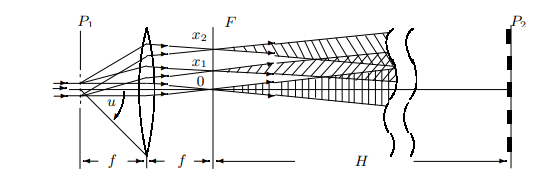
\includegraphics[width=0.6\textwidth]{images/fig1.png}
    \caption{Схема образования изображения в объективе микроскопа.}
    \label{fig:microscope}
\end{figure}

В фокальной плоскости объектива \( F \) формируется дифракционная картина Фраунгофера (первичное изображение). При установке диафрагмы, пропускающей определённые порядки дифракции (\( m = 0, \pm 1 \)), в плоскости \( P_2 \) формируется вторичное изображение. Например:
\begin{itemize}
    \item Вертикальная щель пропускает максимумы \( m_x = 0 \), формируя изображение горизонтальных штрихов.
    \item Горизонтальная щель выделяет \( m_y = 0 \), воспроизводя вертикальные штрихи.
\end{itemize}
Это явление называется \textit{пространственной фильтрацией}.

\subsection*{Критерий разрешения для когерентного освещения}
При уменьшении апертуры \( A \) волны нулевого порядка фокусируются на краю диафрагмы. Для разрешения необходимо, чтобы угол между волнами 0-го и 1-го порядков составлял \( 2u \). Минимальное разрешаемое расстояние:
\begin{equation}
    \ell_{\min} \approx \frac{\lambda}{\sin A} \approx \frac{\lambda}{D / 2f},
\end{equation}
где \( D \) --- диаметр диафрагмы, \( f \) --- фокусное расстояние объектива.

\section*{Экспериментальная установка}

\subsection*{Схема проекционного микроскопа}
\begin{figure}[H]
    \centering
    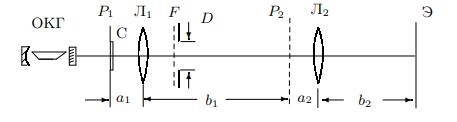
\includegraphics[width=0.7\textwidth]{images/fig3.png}
    \caption{Схема экспериментальной установки: 1 --- лазер (ОКГ), 2 --- сетка, 3 --- объектив \( Л1 \), 4 --- фокальная плоскость \( F \), 5 --- линза \( Л2 \), 6 --- экран.}
    \label{fig:setup}
\end{figure}

Установка включает:
\begin{itemize}
    \item Лазер с коллимированным пучком, падающим на сетку \( C \).
    \item Длиннофокусный объектив \( Л1 \) (\( f \approx 10 \) см) для формирования первичного изображения в плоскости \( F \).
    \item Короткофокусную линзу \( Л2 \), проецирующую изображение на экран.
    \item Кассету с сетками различного периода \( d \).
    \item Щелевые и крисовые диафрагмы в плоскости \( F \).
\end{itemize}

\subsection*{Методика измерений}
\begin{enumerate}
    \item \textbf{Калибровка сеток:}
    \begin{itemize}
        \item \textit{По дифракции Фраунгофера:} Измерение расстояния между максимумами на экране с последующим расчётом периода \( d \) по формуле:
        \begin{equation}
            d = \frac{\lambda f}{y},
        \end{equation}
        где \( y \) --- расстояние между максимумами.
        \item \textit{По увеличенному изображению:} Прямое измерение периода через увеличение микроскопа.
    \end{itemize}
    
    \item \textbf{Определение разрешающей способности:}
    Подбор минимального размера щели в плоскости \( F \), пропускающей максимумы \( m = 0, \pm 1 \). Расчёт апертурного угла \( A \) по формуле:
    \begin{equation}
        \sin A = \frac{D}{2f},
    \end{equation}
    где \( D \) --- размер диафрагмы. Проверка соответствия с теорией через соотношение \( \ell_{\min} \approx \lambda / \sin A \).
    
    \item \textbf{Пространственная фильтрация:}
    \begin{itemize}
        \item Наклон щели позволяет получать изображение наклонной решётки.
        \item Перестановка сетки и щели вызывает мультипликацию изображения.
    \end{itemize}
\end{enumerate}

\subsection*{Особенности установки}
\begin{itemize}
    \item Для безопасности исключено визуальное наблюдение через окуляр.
    \item Наличие непериодического объекта (проволочки) для идентификации геометрического изображения.
    \item Использование крисовой диафрагмы для изменения апертуры.
    \item Возможность установки масок в плоскости \( F \) для демонстрации пространственной фильтрации.
\end{itemize}

\section*{Результаты измерений и обработка данных}

\subsection*{Определение периода решёток по их пространственному спектру}

Соберём установку согласно описанию. Длина волны излучения лазера $\lambda=532 \mathrm{нм}$
Расстояние от сетки до экрана $H=100 \pm 2$ см, погрешность объясняется неопределённостью положения сетки внутри кассеты, погрешностью меток на столе, использованных при измерении, и погрешностью прямого измерения. Измерим линейкой на экране расстояние $\Delta x$ между $n+1$ максимумами и рассчитаем по второй формуле с учётом $\varphi=\frac{\Delta x}{H}$ период решетки $d = \frac{n\lambda}{\Delta x}H$. Результаты приведены в Таблице $1 .$

\begin{minipage}{0.47\textwidth}
\begin{center}
\begin{tabular}{|c|c|c|c|}
\hline
Номер &$\Delta x$, см &  n&$d$, мкм\\
решётки&		&			& \\
\hline
1 &	22.7	&6	& 		20	\\
\hline
2&	22.6	&	9	&	30		\\
\hline
3&	25.1	&20		&	60		\\
\hline
4&	22.5	&	35	&	117		\\
\hline
5&	22.7	&	48	&		159	\\
\hline
\end{tabular}
\newline
\newline
Таблица 1. 
\end{center}
\end{minipage}
\begin{minipage}{0.47\textwidth}
\begin{center}
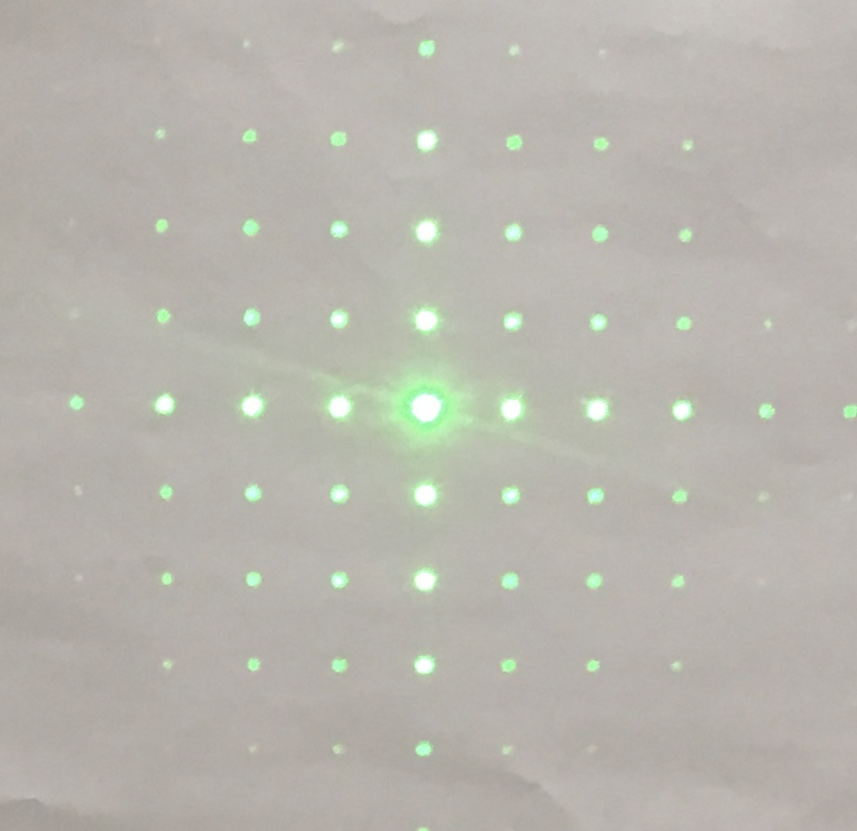
\includegraphics[width = \textwidth]{images/2.jpg}
\end{center}

\begin{center}
Дифракция Фраунгофера на двумерной решетке.
\end{center}
\end{minipage}



 
\subsection*{Определение периода решёток по изображению, увеличенному с помощью модели микроскопа}
  
Соберём модель микроскопа, добавив линзы согласно Рис. 1. Фокусные расстояния линз $F_{1}=  $ мм, $F_{2}= $ мм. Измеряем необходимые расстояния:
$$
\begin{aligned}
a_{1} &= 120  \pm 10 \mathrm{мм}, \\
a_{2}+b_{1} &= 455 \pm 10 \mathrm{см}, \\
b_{2} &= 815 \pm 10 \mathrm{см},
\end{aligned}
$$
Погрешности здесь обусловлены неточностями в положенияъ сеток и линз. Из формулы тонкой линзы \fbox{$a_{2}=\frac{b_{2} F_{2}}{b_{2}-F_{2}}=25.79$ мм}, откуда \fbox{$a_{2} \approx F_{2}$}, поэтому в дальнейшем будем использовать это значение, следовательно $b_{1}= 420\pm 10$ мм.  Увеличение микроскопа \fbox{$ \Gamma=\frac{b_{1} b_{2}}{a_{1} a_{2}}=114 \pm 10 .$}

Повторим измерения периодов изображений в новой конфигурации, погрешности считаются аналогично. Измерение представлены в Таблице $2 .$

Здесь $d$ определялось по формуле $d=\frac{\Delta x}{\Gamma n}$. Обратим внимание, что значения периодов решётки совпадают в пределах погрешности.

\begin{minipage}{0.47\textwidth}
\begin{center}
\begin{tabular}{|c|c|c|c|}
\hline
Номер &$\Delta x$, см &  n&$d$, мкм\\
решётки&		&			& \\
\hline
1 &	3.7	&	16	& 	20		\\
\hline
2&	15.7	&	49	&	28		\\
\hline
3&	25.3	&	38	&	58		\\
\hline
4&	24.1	&	18	&	117		\\
\hline
5&	23.6	&	13	&	159	 	\\
\hline
\end{tabular}
\newline
\newline
Таблица 2. 
\end{center}
\end{minipage}
\begin{minipage}{0.47\textwidth}
\begin{center}
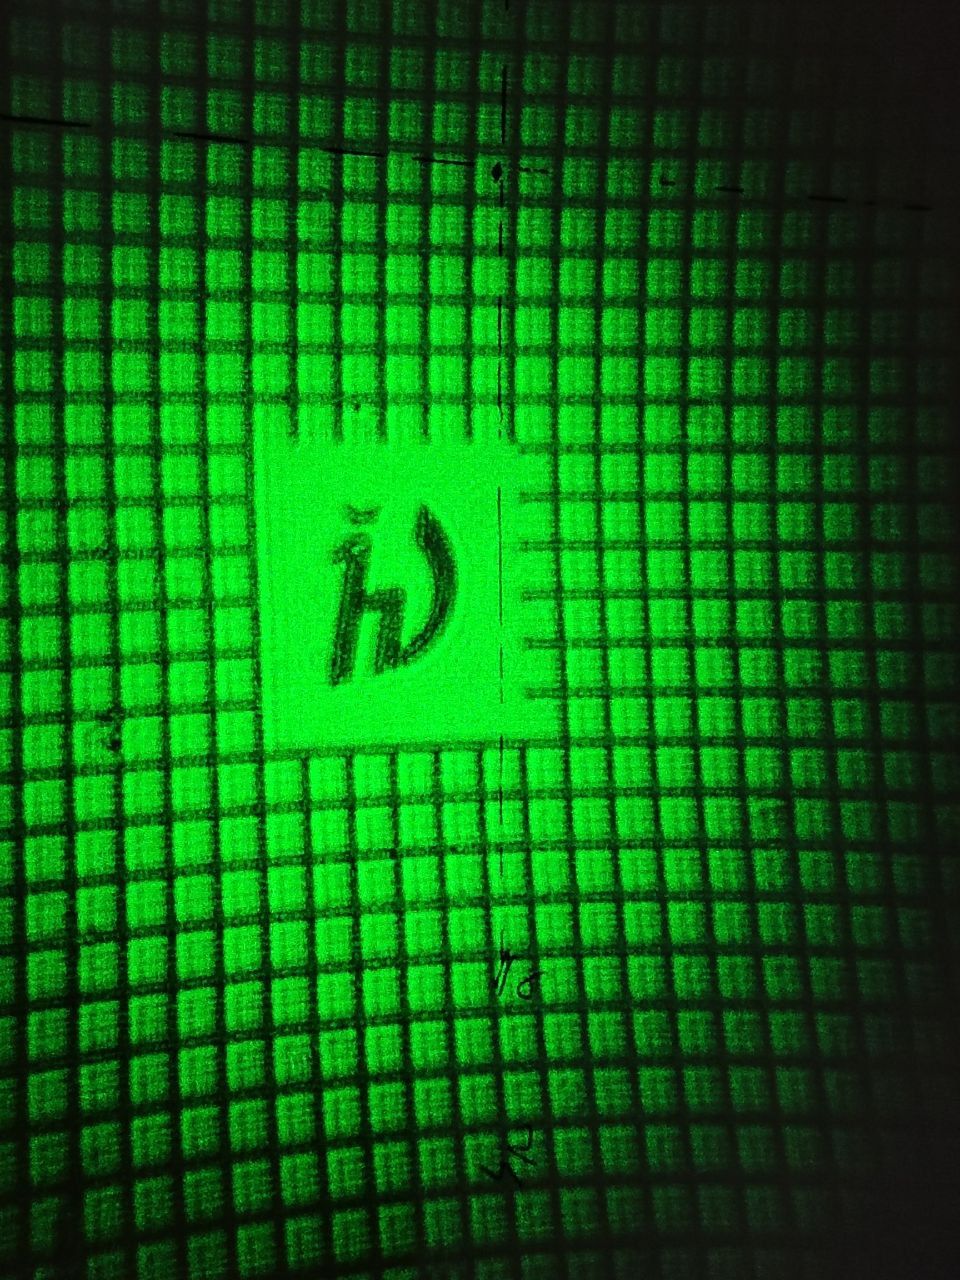
\includegraphics[width = \textwidth]{images/3.jpg}
\end{center}

\begin{center}
Увеличенное изображение сетки.
\end{center}
\end{minipage}

\subsection*{Определение периода решёток по оценке разрешающей способности микроскопа}

Поместим в фокальной плоскости линзы $Л_{1}$ щелевую диафрагму с микрометрическим винтом и определим минимальную толщину $D$ при которой на экране видна двумерная решётка. В этом случае период будет вычисляться по формуле (3) в предельном случае
$$
d=\frac{2 \lambda F_{1}}{D}
$$
погрешность вычисляется по формуле
$$
\sigma_{d}=d \frac{\sigma_{D}}{D} .
$$
Результаты приведены в Таблице $3 .$



\begin{minipage}{0.47\textwidth}
\begin{center}
\begin{tabular}{|c|c|c|c|}
\hline
Номер &D , мм &  1/D, мм&$d$, мкм\\
решётки&		&			& \\
\hline
1 &--		&	--	& 		--	\\
\hline
2&	4.14	&	0.242	&	28.3		\\
\hline
3&	1.96	&	0.510	&	59.7		\\
\hline
4&	1.02	&	0.980	&	114.7		\\
\hline
5&	0.81	&	1.240	&		144.5	\\
\hline
\end{tabular}
\newline
\newline
Таблица 3. 
\end{center}
\end{minipage}
\begin{minipage}{0.47\textwidth}
\begin{center}
		\begin{tikzpicture}[scale = 1.0]
		\begin{axis}[
		axis lines = left,
		ylabel = {d, мкм},
		xlabel = {1/D, мм},
		minor grid style={black, line width=0.05pt},
		major grid style={solid,black, line width=0.3pt},
		xmin=0, xmax=1.4,
		ymin=0, ymax=160,
		ymajorgrids = true,
		xmajorgrids = true,
		yminorgrids = true,
		xminorgrids = true,
		minor tick num = 4
		]
		\addplot+[only marks ] plot[error bars/.cd, y dir=both, y explicit]
		coordinates {
			(0.242,28.3)
			(0.510,59.7)
			(0.980,114.7)
			(1.24,144.5)
		};
		
		\addplot[blue, domain=0:8]{120.43*x };
		\end{axis}

		\end{tikzpicture}

Зависимость $d=f(1 / D)$. 
		
\end{center}
\end{minipage}

\newline
\newline


Через щель проходили только нулевой (по центру) и два первых максимумы, за исключением второй щели, где нулевой максимум был помещён к краю щели. Для первой решётки
период таким методом измерить не получилось, так как ширины щели не хватает.

Для проверки теории Аббе построим график $d=f\left(\frac{1}{D}\right)$ со значениями $d$ из части 1, погрешность $\frac{1}{D}$ рассчитывается по формуле
$$
\sigma_{1 / D}=\frac{\sigma_{D}}{D^{2}}
$$
Угловой коэффициент прямой из $\mathrm{MHK}\ k=(124 \pm 8) \cdot 10^{-9} м^{2}$, в пределах погрешности он совпадает с теоретическим $2 \lambda F_{1}= 117\cdot 10^{-9} м^{2} .$ Таким образом, теория Аббе подтвердилась. 
   
 \subsection*{Пространственная фильтрация и мультиплицирование}
 
 Для наблюдения фильтрации на сетке 2 откроем щель так, чтобы она пропускала только максимум нулевого порядка и, поворачивая щель, наблюдаем за изменением картины. Картины представлены на рисунках ниже. \\
 
 \begin{minipage}{0.40\textwidth}
\begin{center}
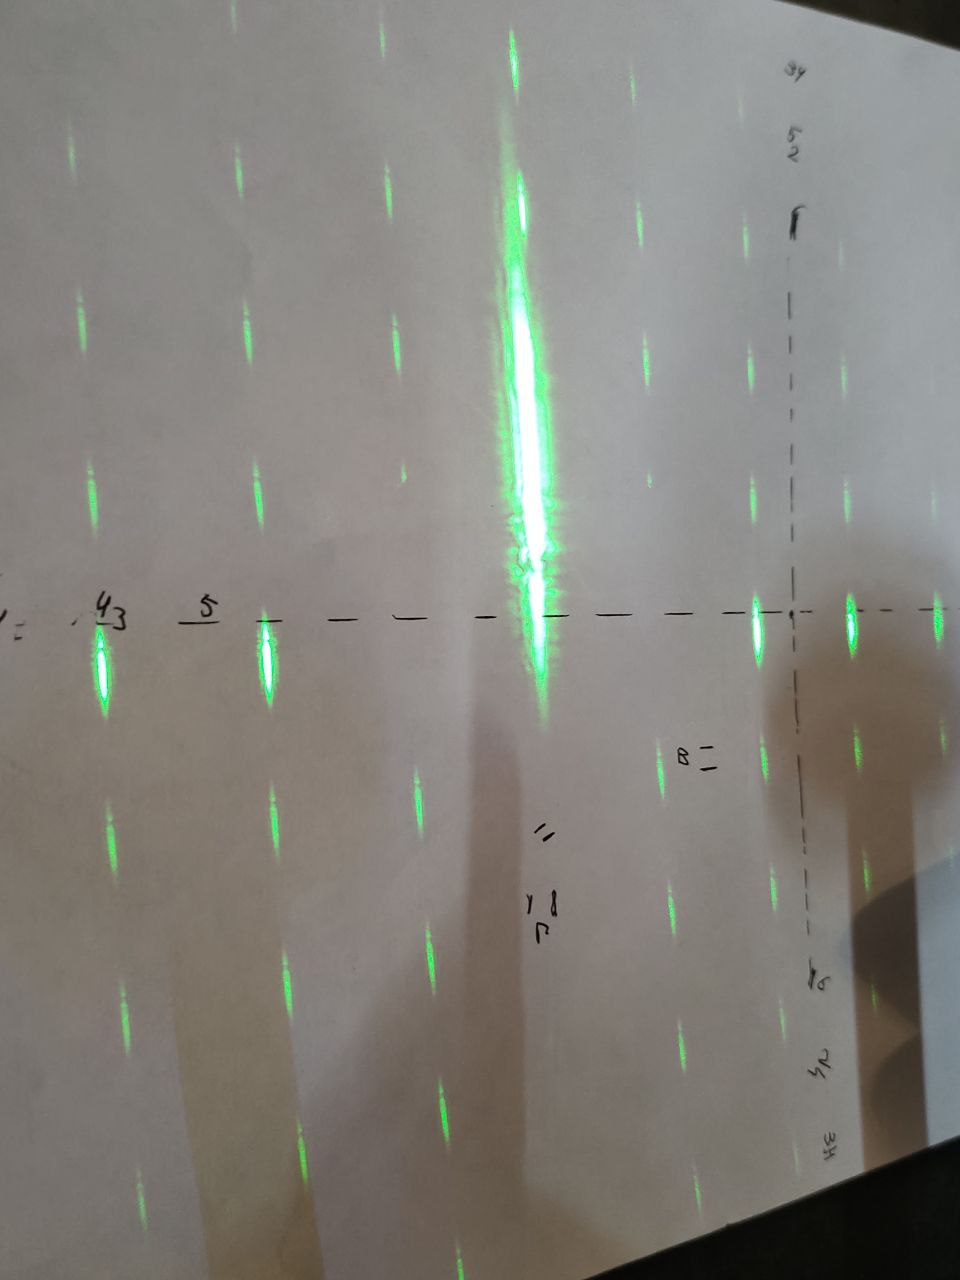
\includegraphics[width = \textwidth]{images/4.jpg}
\end{center}

\begin{center}
Горизонатальная щель $\left(0, m_{y}\right)$. 
\end{center}
\end{minipage}
\begin{minipage}{0.40\textwidth}
\begin{center}
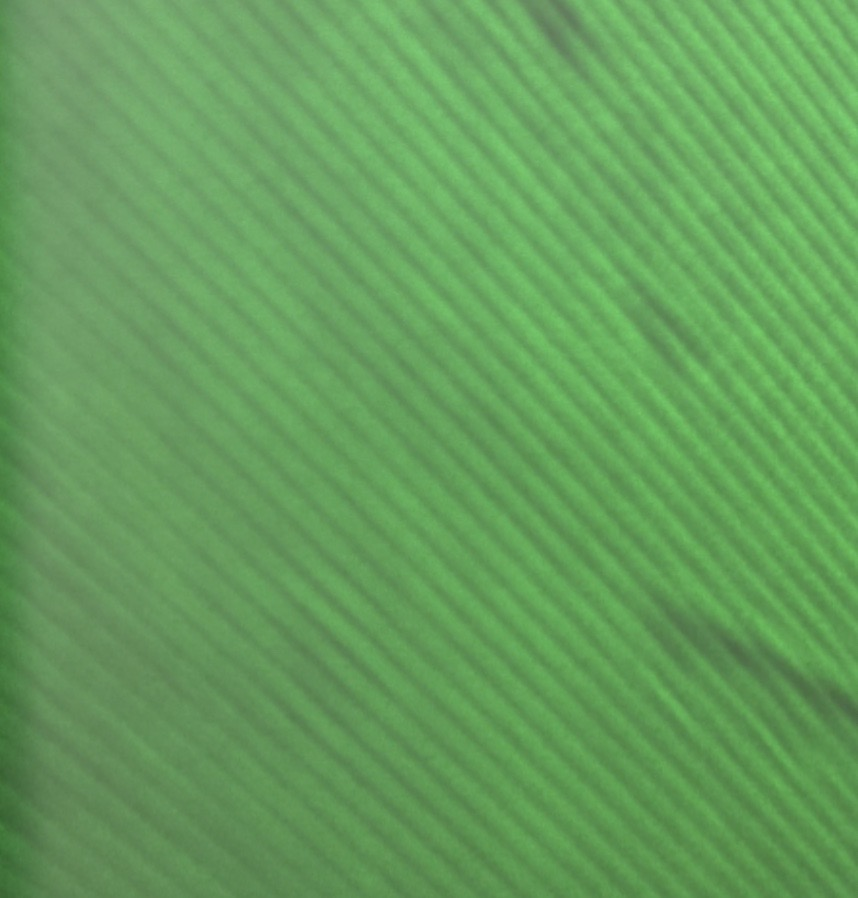
\includegraphics[width = 0.95\textwidth]{images/6.jpg}
\end{center}

\begin{center}
Щель, повернутая на $45^{\circ}\left(m_{x}=m_{y}\right)$. 
\end{center}
\end{minipage}
 
 
 \begin{minipage}{0.40\textwidth}
\begin{center}
 Для наблюдения мультиплицированния поменяем местами сетку и щель, пронаблюдаем мультипликацию, картина представлена на Рис. $4 .$

\end{center}
\end{minipage}
\begin{minipage}{0.40\textwidth}
\begin{center}

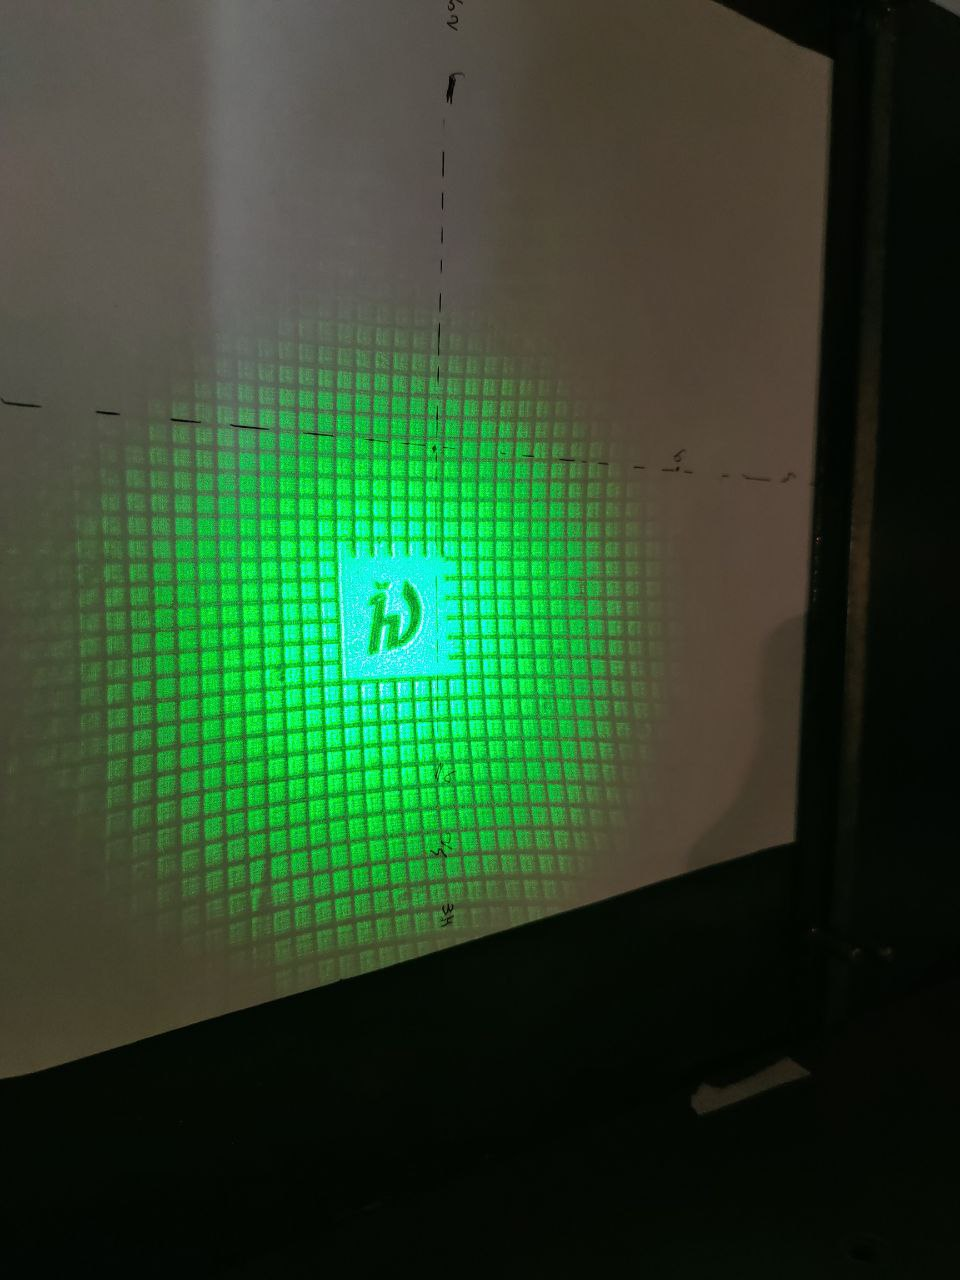
\includegraphics[width = \textwidth]{images/5.jpg}
\end{center}

\begin{center}
Схема для наблюдения интерфереционной картины.

\end{center}
\end{minipage}
\section*{Вывод}

По измерениям спектров определены дифракционные углы и по теоретическим формулам рассчитаны периоды решеток. Полученные данные сошлись с результатами, полученными по измерениям увеличенных с помощью микроскопа изображений сеток. Построен график зависимости d = f(1/D).


\end{document}
